\tikzstyle{block} = [rectangle, draw, fill=blue!20, text centered]
\begin{center}
	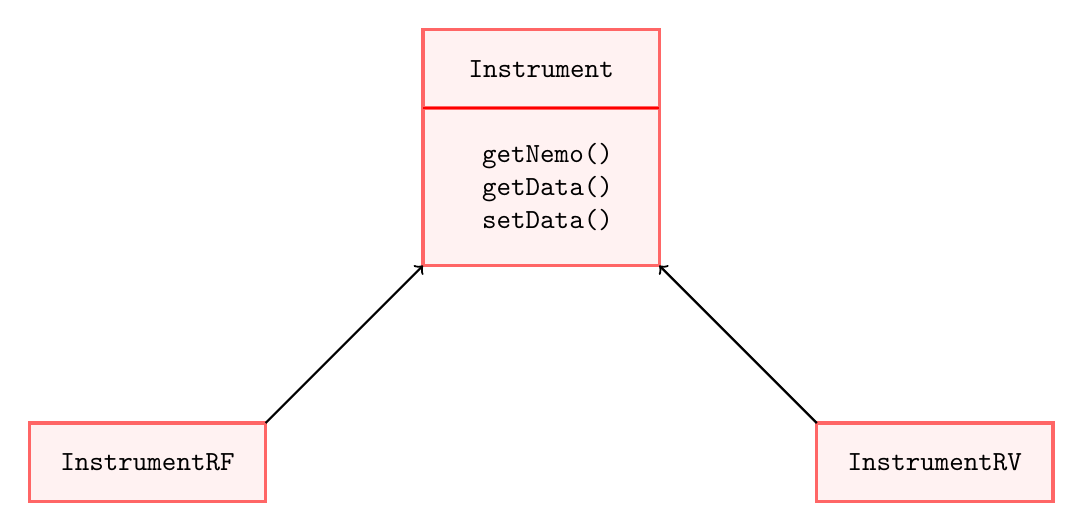
\begin{tikzpicture}
		%\node [block] (madre) {Instrument};
		%\node [block, below of=madre] {InstrumentRV};
		% Cajas
		\filldraw[color=red!60, fill=red!5, very thick] (0,0) rectangle (3,2);
		\filldraw[color=red!60, fill=red!5, very thick] (0,2) rectangle (3,3);
		\draw[thick, red, -] (0,2) -- (3,2);
		% Tamaños de las cajas
		\node[] at (1.5,2.5) {\texttt{Instrument}};
		\node[text width=1.5cm,text centered] at (1.5,1) {
			\texttt{getNemo()}
			\texttt{getData()}
			\texttt{setData()}
		};
		\filldraw[color=red!60, fill=red!5, very thick] (-5,-3) rectangle (-2,-2);
		\node[] at (-3.5,-2.5) {\texttt{InstrumentRF}};
		\filldraw[color=red!60, fill=red!5, very thick] (5,-3) rectangle (8,-2);
		\node[] at (6.5,-2.5) {\texttt{InstrumentRV}};
		\draw[->, thick] (-2,-2) -- (0,0);
		\draw[->, thick] (5,-2) -- (3,0);
	\end{tikzpicture}
\end{center}